\documentclass[11pt,a4paper]{article}
\usepackage[utf8]{inputenc}
\usepackage[T1]{fontenc}
\usepackage[margin=1in]{geometry}
\usepackage{xcolor}
\usepackage{tcolorbox}
\usepackage{booktabs}
\usepackage{pgfplots}
\usepackage{graphicx}
\pgfplotsset{compat=1.18}
\usepackage{sectsty}
\usepackage{mathpazo} 

\definecolor{brandblue}{HTML}{0D47A1}
\definecolor{goodgreen}{HTML}{2E7D32}
\definecolor{badred}{HTML}{C62828}
\definecolor{surface}{HTML}{F8F9FA}
\sectionfont{\color{brandblue}}

\begin{document}
\begin{center}
{\Huge\bfseries\color{brandblue} Full-Spectrum Trading Analytics}\\[0.5em]
{\Large Complete Tier Analysis Report}\\[1em]
{\large Prepared for \textbf{Mission Credit Card}}\\[0.5em]
{\small Generated on \today}
\end{center}
\vspace{1em}

% >>> FREE TIER
\section*{Free Tier: Trade Log Transparency}
\begin{tcolorbox}[colframe=brandblue, colback=surface, title=Free Tier Headline, fonttitle=\bfseries]
\begin{tabular}{p{0.3\textwidth} p{0.3\textwidth} p{0.3\textwidth}}
\textbf{Total Net P\&L} & \textbf{Win Rate} & \textbf{Profit Factor} \\
{\Large \color{badred} \$-715.16} & {\Large 25.0\%} & {\Large 0.66} \\
\end{tabular}\\[1em]
\textbf{Total Trades:} 28 \quad \textbf{Expectancy:} \$-25.54 \quad \textbf{Avg Win/Loss:} \$202.67 / \color{badred}\$101.61
\end{tcolorbox}

\vspace{0.5em}
\noindent\textbf{Direction Split:}\\
\begin{tabular}{@{} l r r l r @{}}
\toprule
\textbf{Direction} & \textbf{Trades} & \textbf{Win Rate} & \textbf{Net P\&L} & \textbf{Profit Factor} \\
\midrule

\textbf{Buy (*)} & 11 & 27.3\% & \color{goodgreen}\$17.84 & 1.02 \\

\textbf{Sell} & 17 & 23.5\% & \color{badred}\$-733.00 & 0.44 \\

\bottomrule
\end{tabular}

\vspace{1em}
\noindent\textbf{Session Heatmap (Net P\&L by Entry Hour):}\\
\begin{center}
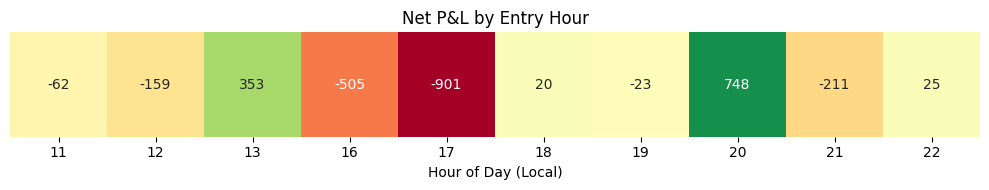
\includegraphics[width=0.9\textwidth]{session_heatmap.png}
\end{center}

\newpage
% >>> TIER 1
\section*{Tier 1: Edge Tracker}
\subsection*{Hold Time Analysis}
\begin{tabular}{@{} l r r r l r @{}}
\toprule
\textbf{Bucket} & \textbf{Trades} & \textbf{\% All} & \textbf{Win Rate} & \textbf{Net P\&L} & \textbf{Profit Factor} \\
\midrule

\textbf{Scalp} & 7 & 25.0\% & 0.0\% & \color{badred}\$-665.44 & 0.00 \\

\textbf{Short} & 10 & 35.7\% & 10.0\% & \color{badred}\$-870.18 & 0.10 \\

\textbf{Medium} & 9 & 32.1\% & 44.4\% & \color{goodgreen}\$684.94 & 2.36 \\

\textbf{Long} & 2 & 7.1\% & 100.0\% & \color{goodgreen}\$135.52 & inf \\

\bottomrule
\end{tabular}

\vspace{1em}
\subsection*{Entry Quality Score (Proxy MFE/MAE)}
Average absolute friction (spread+slippage+fees) cost per trade: \textbf{\$1.72 (2.4\% of gross move)}

\vspace{1em}
\subsection*{Streak Tracker}
\begin{tabular}{l l | l l}
\textbf{Max Win Streak:} & 2 & \textbf{Avg Win Streak:} & 1.2 \\
\textbf{Max Loss Streak:} & 5 & \textbf{Avg Loss Streak:} & 3.0 \\
\end{tabular}
\vspace{1em}
\begin{center}
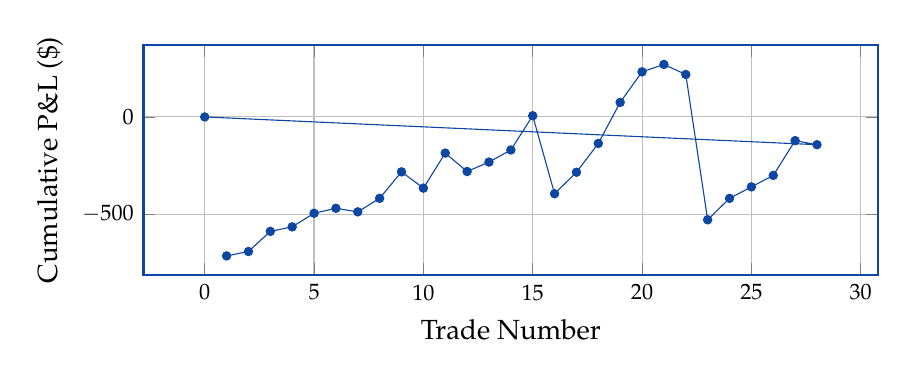
\begin{tikzpicture}
\begin{axis}[
    width=0.9\textwidth, height=4.5cm, grid=major,
    xlabel={Trade Number}, ylabel={Cumulative P\&L (\$)},
    axis line style={brandblue, thick}, x tick label style={font=\footnotesize}, y tick label style={font=\footnotesize}
]
\addplot[color=brandblue, mark=*, mark size=1.5pt] coordinates { (0, 0) (28, -142.86) (27, -121.98) (26, -300.84) (25, -359.96) (24, -419.08) (23, -529.32) (22, 218.44) (21, 270.20) (20, 232.08) (19, 74.84) (18, -136.40) (17, -284.64) (16, -395.26) (15, 6.12) (14, -170.12) (13, -232.24) (12, -280.86) (11, -186.10) (10, -366.34) (9, -282.58) (8, -418.82) (7, -488.44) (6, -470.06) (5, -495.68) (4, -565.80) (3, -588.92) (2, -692.54) (1, -715.16) };
\end{axis}
\end{tikzpicture}
\end{center}

\vspace{1em}
% >>> TIER 2
\section*{Tier 2: Pattern Intelligence}
\subsection*{Best Setup Detector (N $\geq$ 3)}
\begin{tabular}{@{} l l l l r l r @{}}
\toprule
\textbf{Dir} & \textbf{Session} & \textbf{Duration} & \textbf{Size} & \textbf{Trades} & \textbf{Win Rate} & \textbf{Expectancy} \\
\midrule

\bottomrule
\end{tabular}

\vspace{1em}
\subsection*{Tilt Detection (Behavioral Flags)}
\begin{itemize}
\item \textbf{Rapid Re-entry Clusters} ($<$ 30m after loss): 0
\item \textbf{Size Escalations} (immediately after loss): 2
\item \textbf{Est. P\&L Impact of Tilt Trades}: \color{badred}\$-62.48
\end{itemize}

\newpage
% >>> TIER 3
\section*{Tier 3: Coaching Layer}
\subsection*{Personalised Regime Detection}
\begin{tabular}{@{} l l r l @{}}
\toprule
\textbf{Date} & \textbf{Regime} & \textbf{Trades} & \textbf{Session P\&L} \\
\midrule

2026-02-23 & Trending & 2 & \color{badred}\$-121.98 \\

2026-02-24 & Trending & 2 & \color{badred}\$-237.98 \\

2026-02-25 & Low Sample & 1 & \color{badred}\$-59.12 \\

2026-02-26 & Volatile & 2 & \color{goodgreen}\$637.52 \\

2026-02-27 & Low Sample & 1 & \color{goodgreen}\$51.76 \\

2026-03-02 & Trending & 2 & \color{badred}\$-195.36 \\

2026-03-03 & Low Sample & 1 & \color{badred}\$-211.24 \\

2026-03-04 & Low Sample & 1 & \color{badred}\$-148.24 \\

2026-03-06 & Low Sample & 1 & \color{badred}\$-110.62 \\

2026-03-10 & Volatile & 2 & \color{goodgreen}\$225.14 \\

2026-03-11 & Mixed & 3 & \color{badred}\$-15.98 \\

2026-03-12 & Trending & 2 & \color{badred}\$-96.48 \\

2026-03-13 & Mixed & 2 & \color{badred}\$-205.86 \\

2026-03-16 & Trending & 2 & \color{badred}\$-7.24 \\

2026-03-18 & Low Sample & 1 & \color{badred}\$-70.12 \\

2026-03-20 & Low Sample & 1 & \color{badred}\$-23.12 \\

2026-03-24 & Trending & 2 & \color{badred}\$-126.24 \\

\bottomrule
\end{tabular}

\vspace{1em}
\subsection*{Monte Carlo Risk Sizing}
Simulating 10,000 paths of 100 trades based on your historical P\&L distribution, with a \$10,000 starting account and \$1,000 drawdown threshold.\\

\vspace{0.5em}
\begin{tabular}{l l l l}
\textbf{Median Final P\&L:} & \$-2649.35 & \textbf{5th Percentile:} & \$-5543.41 \\
\textbf{95th Percentile:} & \$702.38 & \textbf{Prob of Ruin:} & \textbf{\color{badred}91.6\%} \\
\end{tabular}
\begin{center}
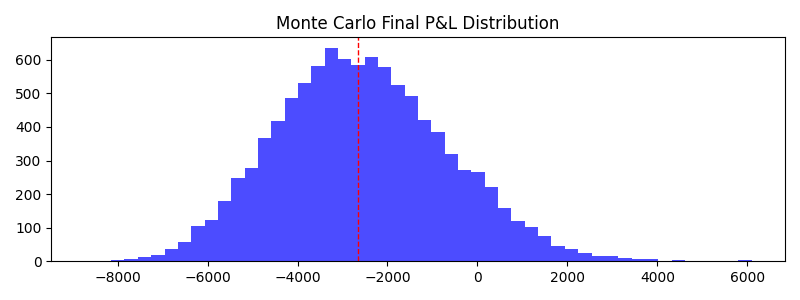
\includegraphics[width=0.75\textwidth]{monte_carlo.png}
\end{center}

\vspace{1em}
\subsection*{Custom Rule Alerts}

The following system violations were flagged based on \texttt{rules.json}:\\

\begin{tabular}{@{} l r l @{}}
\toprule
\textbf{Rule Breached} & \textbf{Count} & \textbf{P\&L Impact} \\
\midrule

SIZE\_LIMIT & 2 & \color{badred}\$-321.72 \\

\bottomrule
\end{tabular}


\vspace{1em}
\subsection*{Actionable Coaching Directives}
\begin{tcolorbox}[colframe=badred!80!black, colback=surface, title=Critical Focus Areas]
\begin{itemize}

\item \textbf{Directional Bias:} Your edge is heavily skewed towards \textbf{Buy} setups. Consider taking 50\% size or skipping opposite direction signals completely.

\item \textbf{Psychology Leak:} Data shows revenge trading patterns (0 fast re-entries, 2 size escalations). Implement a mandatory 15-minute screen break after any loss.

\item \textbf{Capital Preservation:} Your Probability of Ruin is dangerously high (91.6\%!). To survive statistical variance, reduce your standard contract size immediately until the curve smooths out.

\item \textbf{Discipline Breach:} You broke your system rules (SIZE\_LIMIT). An edge is mathematically meaningless without compliance. Focus solely on execution tomorrow, not P\&L.

\end{itemize}
\end{tcolorbox}

\end{document}